\documentclass[12pt,titlepage]{article}
\usepackage[margin=1.25in]{geometry}
\usepackage{graphicx,amsmath,blindtext,minted}

%% Variables definition
\newcommand{\vSubject}{Mathematics 3}
\newcommand{\vSubtitle}{Tree}
\newcommand{\vName}{Muhammad Baihaqi Aulia Asy'ari}
\newcommand{\vNIM}{2241720145}
\newcommand{\vClass}{2I}
\newcommand{\vDepartment}{Information Technology}
\newcommand{\vStudyProgram}{D4 Informatics Engineering}

%% [START] Tikz related stuff
\usepackage{tikz}
\usetikzlibrary{svg.path,calc,shapes.geometric,shapes.misc}
\tikzstyle{terminator} = [rectangle, draw, text centered, rounded corners = 1em, minimum height=2em]
\tikzstyle{preparation} = [chamfered rectangle, chamfered rectangle sep=0.75em, draw, text centered, minimum height = 2em]
\tikzstyle{process} = [rectangle, draw, text centered, minimum height=2em]
\tikzstyle{decision} = [diamond, aspect=2, draw, text centered, minimum height=2em]
\tikzstyle{data}=[trapezium, draw, text centered, trapezium left angle=60, trapezium right angle=120, minimum height=2em]
\tikzstyle{connector} = [line width=0.25mm,->]
%% [END] Tikz related stuff

%% [START] Fancy header related stuff
\usepackage{fancyhdr}
\pagestyle{fancy}
\setlength{\headheight}{15pt} % compensate fancyhdr style
\fancyhead{}
\fancyfoot{}
\fancyfoot[L]{\thepage}
\fancyfoot[R]{\textit{\vSubject - \vSubtitle}}
\renewcommand{\footrulewidth}{0.4pt}% default is 0pt, overline for footer
%% [END] Fancy header related stuff

%% [START] Custom tabular command related stuff
\usepackage{tabularx}
\newcommand{\details}[2]{
    #1 & #2  \\
}
%% [END] Custom tabular command related stuff

%% [START] Figure related stuff
\newcommand{\image}[3][1]{
    \begin{figure}[h]
        \centering
        \includegraphics[#1]{#2}
        \caption{#3}
        \label{#3}
    \end{figure}
}
%% [END] Figure related stuff

%%
\usepackage{pgf-umlcd}

\renewcommand{\umldrawcolor}{black}
\renewcommand{\umlfillcolor}{white}
%%

%% [BEGIN] Custom enumerator
\usepackage{enumitem}
%% [END] Custom enumerator

%% [BEGIN] Paragraph indent
\usepackage{indentfirst}
%% [END] Paragraph indent

%% [BEGIN] URL
\usepackage{hyperref}
\hypersetup{
    colorlinks=true,
    linkcolor=blue,
    filecolor=magenta,      
    urlcolor=cyan,
    pdftitle={Overleaf Example},
    pdfpagemode=FullScreen,
    }

\urlstyle{same}
%% [END] URL

\begin{document}
\begin{titlepage}
    \centering
    \vfill
    {\bfseries\LARGE
        \vSubject\\
        \vskip0.25cm
        \vSubtitle
    }
    \vfill
    
\includegraphics[width=6cm]{images/polinema-logo.png}
    \vfill
    {
        \textbf{Group Members}\\
        \vspace{0.5cm}
        \begin{tabular}{l l}
            Azahra Salsabila & \textbf{2241720073} \\
            Gastiadirijal Naufaldy Kestiyanto & \textbf{2241720001} \\
            Malik Abdul Azis & \textbf{2241720240}\\
            Muhammad Baihaqi Aulia Asy'ari & \textbf{2241720145} \\
        \end{tabular}
        \vskip0.5cm
        \textbf{Class}\\
        \vClass\\
        \vskip0.5cm
        \textbf{Department}\\
        \vDepartment\\
        \vskip0.5cm
        \textbf{Study Program}\\
        \vStudyProgram
    }
\end{titlepage}

\newpage

\section*{Task 1}
Which of the follwing images is a tree graph?
\begin{center}
    \includegraphics[width=.6\textwidth]{images/figures/fig1.png}
\end{center}

\subsection*{Answer}
C. because to be considered as a tree, a graph must have these properties: any pair of vertices connected to each other must not have any same relation to another vertices except for their relation to each other, the number of edges must be 1 less than the number of vertex the graph has, and the relation between vertex must be undirected and interconnected to each other. in other word a graph must not have circuits within it self, must have edges n-1 to the number of vertex and have all vertex interconnected without direction of edges to be considered as a tree graph.  

\newpage

\section*{Task 2}
Find the minimum spanning tree from the following image with the prim algorithm, continue the table below
\begin{center}
    \includegraphics[width=.6\textwidth]{images/figures/fig2.png}\\
    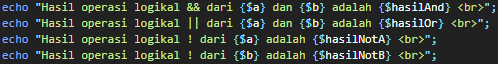
\includegraphics[width=.8\textwidth]{images/figures/fig3.png}\\
\end{center}

\subsection*{Answer}
\resizebox{.9\textwidth}{!}{
    \begin{tabular}{|m{.1\textwidth}|m{.1\textwidth}|m{.1\textwidth}|m{.5\textwidth}|}
        \hline
        Langkah & sisi & bobot & pohon merintang \\ 
        \hline
        1 & (f,g) & 2 & \includegraphics[width=.45\textwidth]{images/figures/fig4.png} \\ 
        \hline
        2 & (f,e) & 3 & 
\includegraphics[width=.45\textwidth]{images/figures/fig5.png} \\ 
        \hline
        3 & (g,h) & 4 & 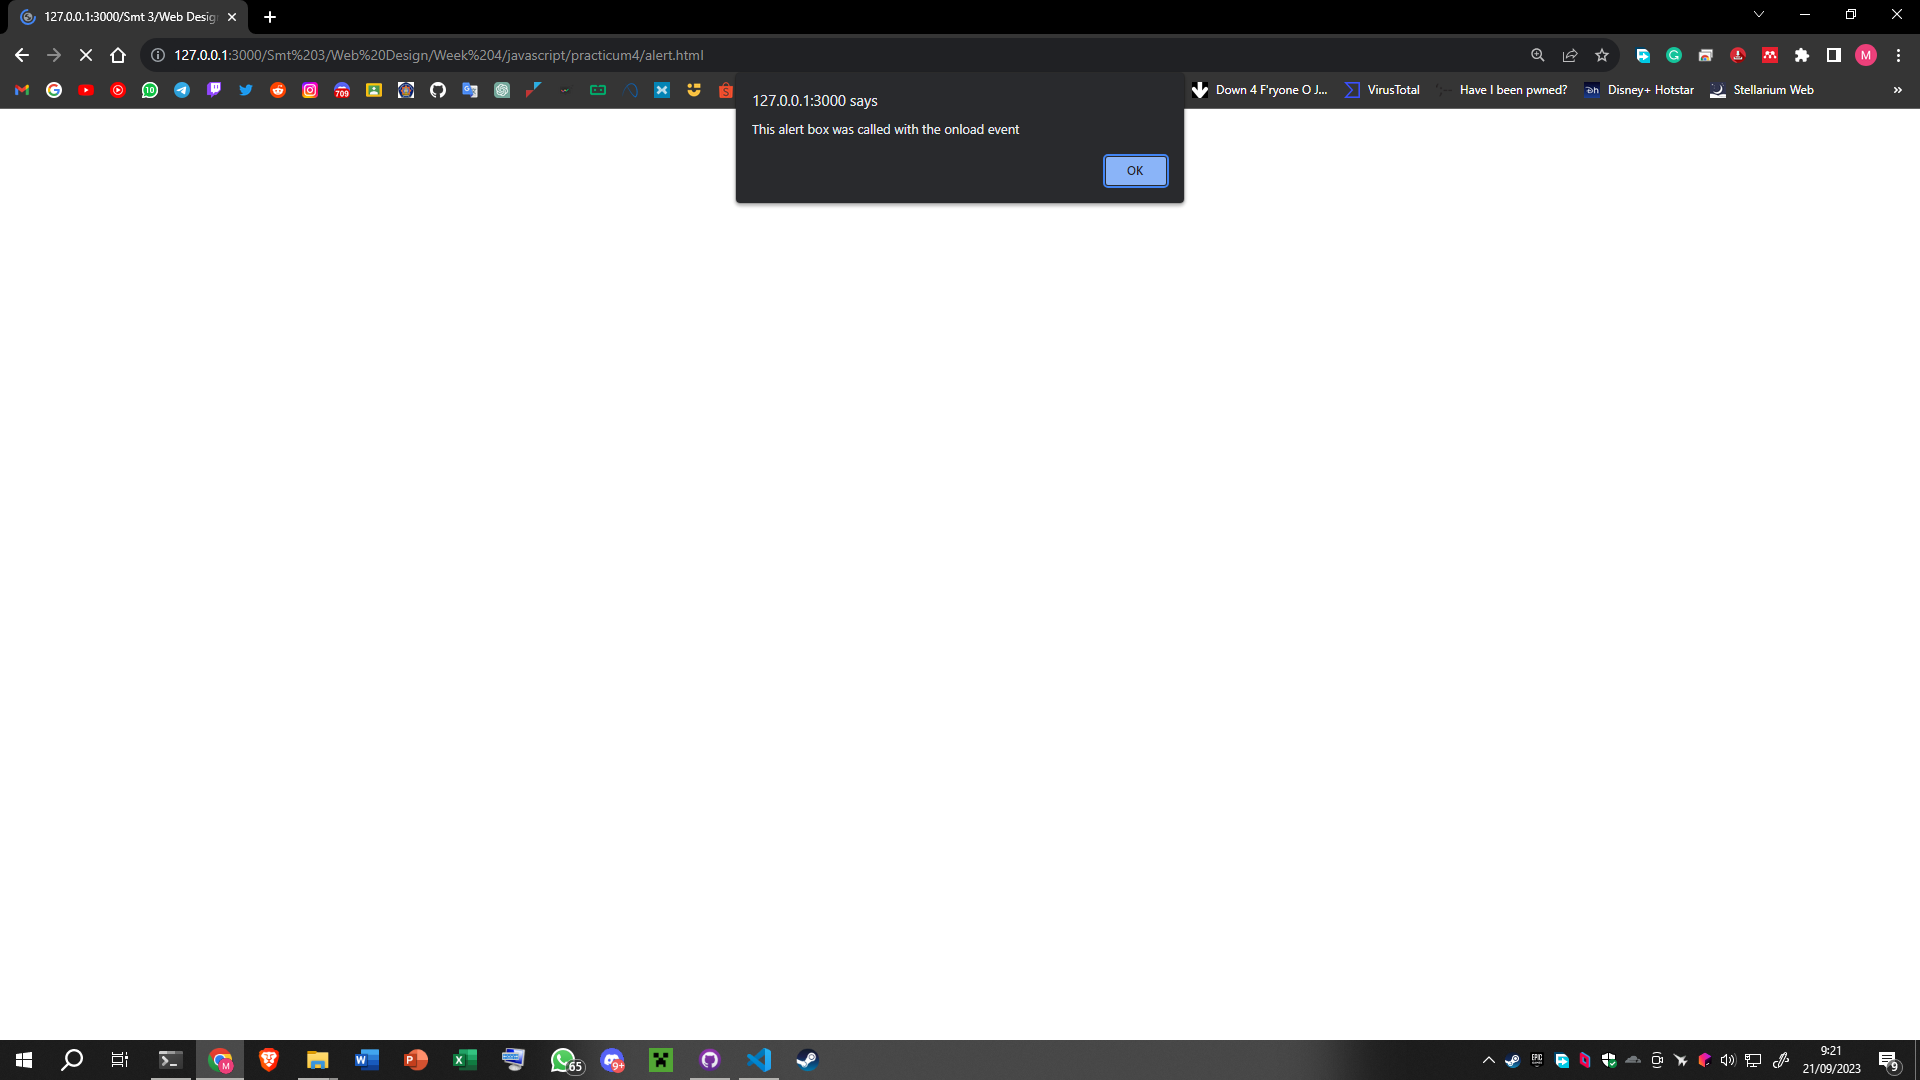
\includegraphics[width=.45\textwidth]{images/figures/fig6.png} \\ 
        \hline
    \end{tabular}
}
\newpage
\resizebox{.9\textwidth}{!}{
    \begin{tabular}{|m{.1\textwidth}|m{.1\textwidth}|m{.1\textwidth}|m{.5\textwidth}|}
        \hline
        4 & (e,a) & 4 & \includegraphics[width=.45\textwidth]{images/figures/fig7.png} \\ 
        \hline
        5 & (a,d) & 4 & \includegraphics[width=.45\textwidth]{images/figures/fig8.png} \\ 
        \hline
        6 & (a,c) & 4 & 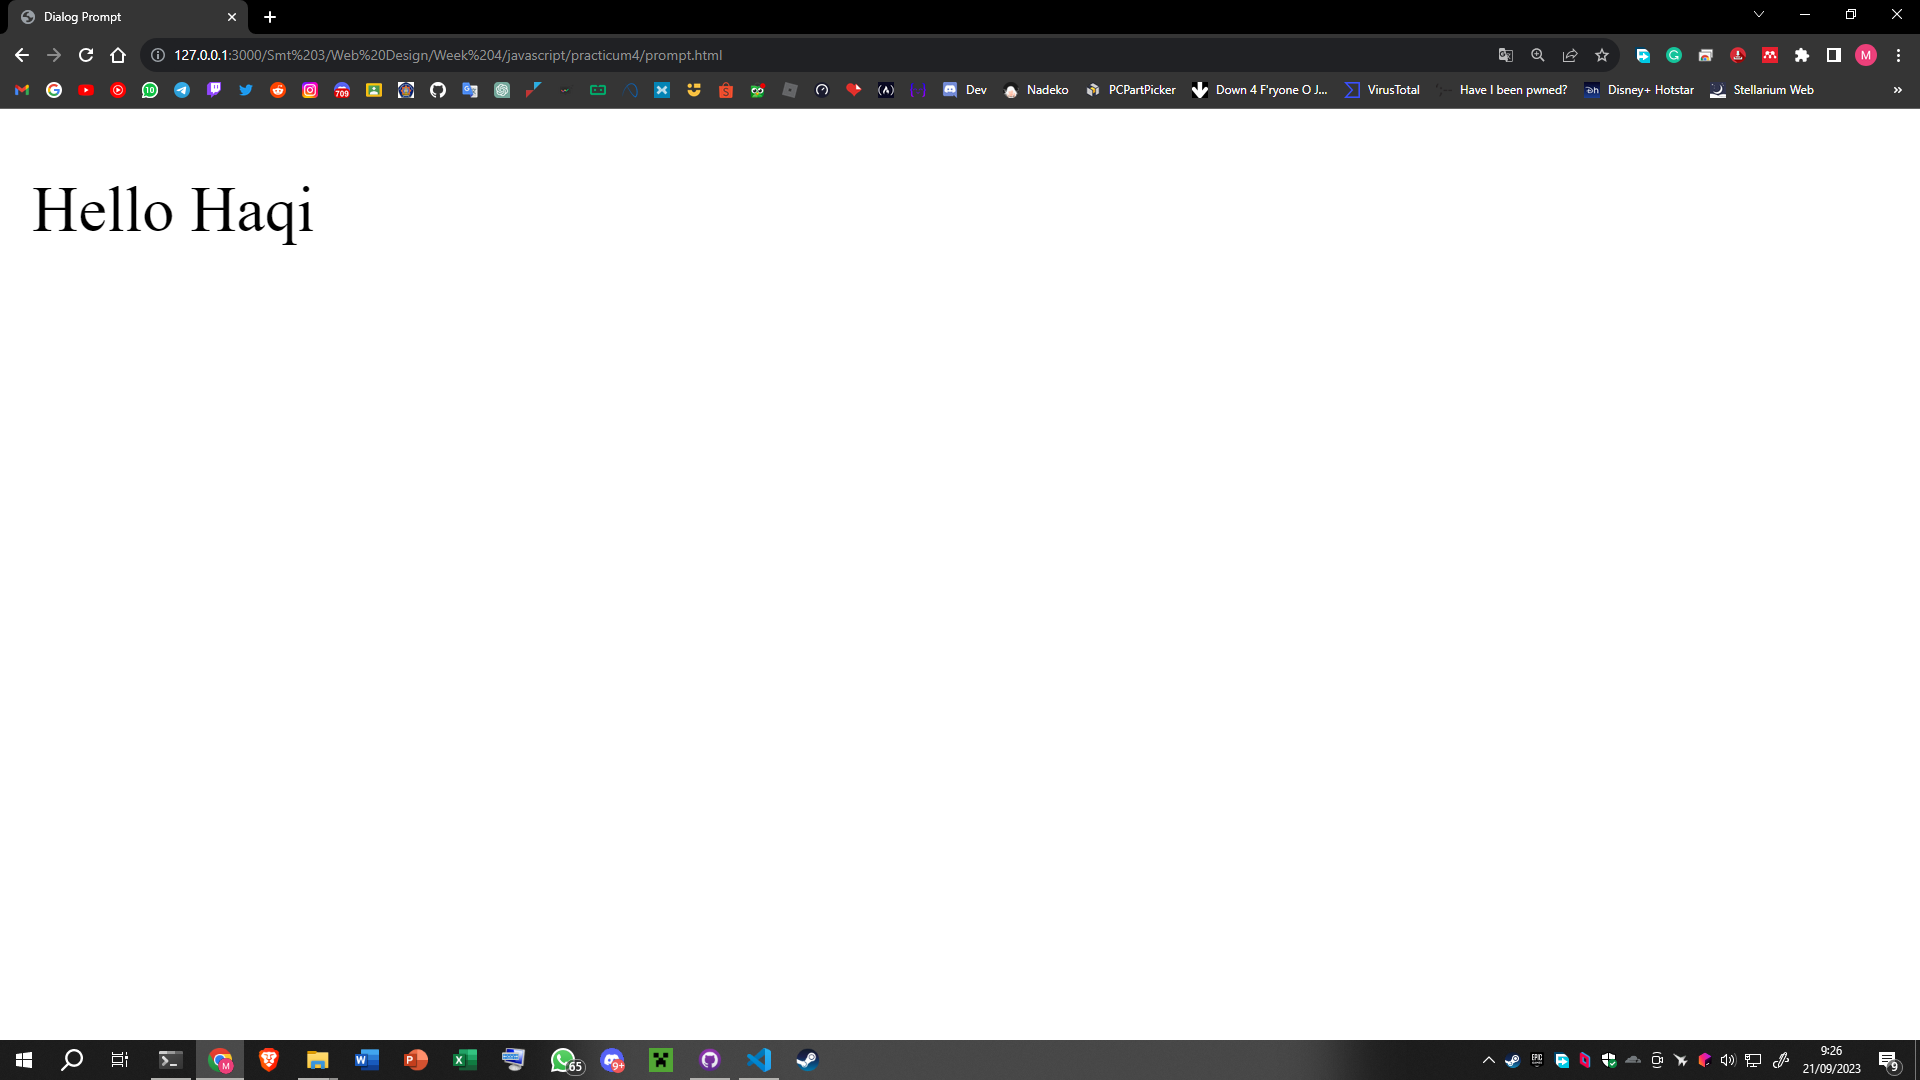
\includegraphics[width=.45\textwidth]{images/figures/fig9.png} \\ 
        \hline
    \end{tabular}
}
\newpage
\resizebox{.9\textwidth}{!}{
    \begin{tabular}{|m{.1\textwidth}|m{.1\textwidth}|m{.1\textwidth}|m{.5\textwidth}|}
        \hline
        7 & (c,b) & 3 & 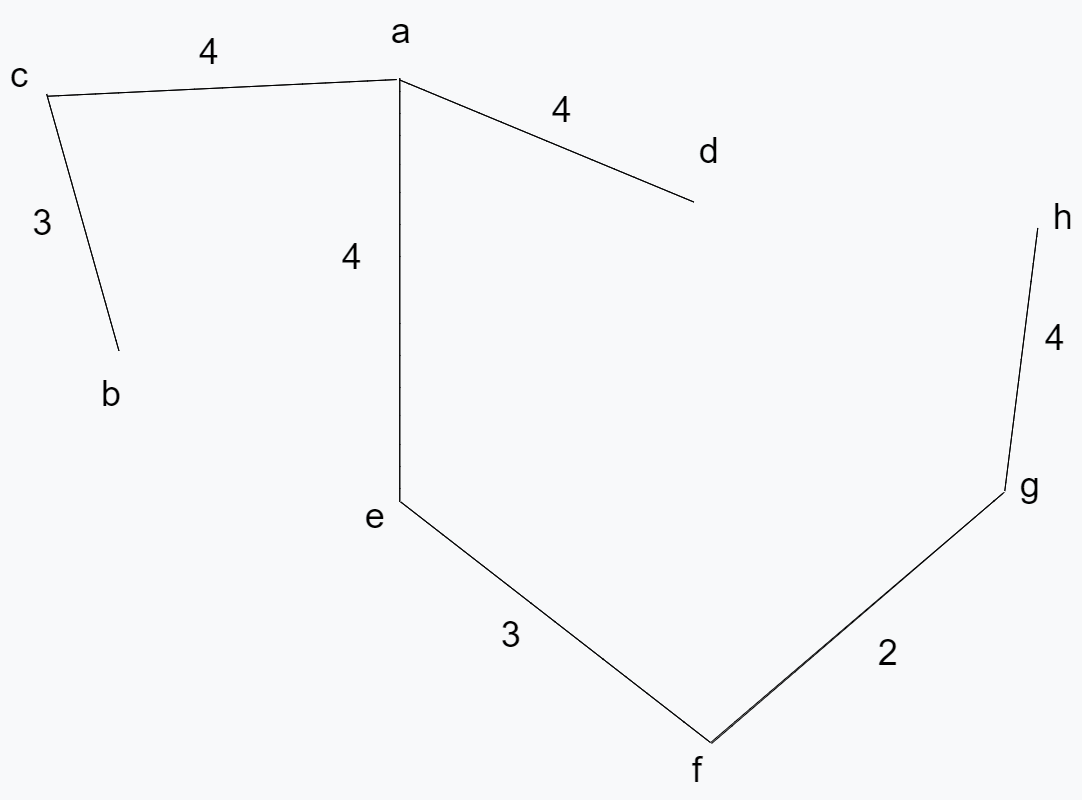
\includegraphics[width=.45\textwidth]{images/figures/fig10.png} \\ 
        \hline
    \end{tabular}
}
\newpage

\section*{Task 3}
Look for 1 example of a journal application of a Tree / Decision tree and draw a picture of the tree arrangement 

\subsection*{Answer}
in the journal article titled \textbf{"Pemilihan Supplier Bahan Baku Kertas Dengan Model QCDFR dan Analytical Hierarchy Process (AHP)"}, a weighted rooted tree graph is used to measure company performance. 

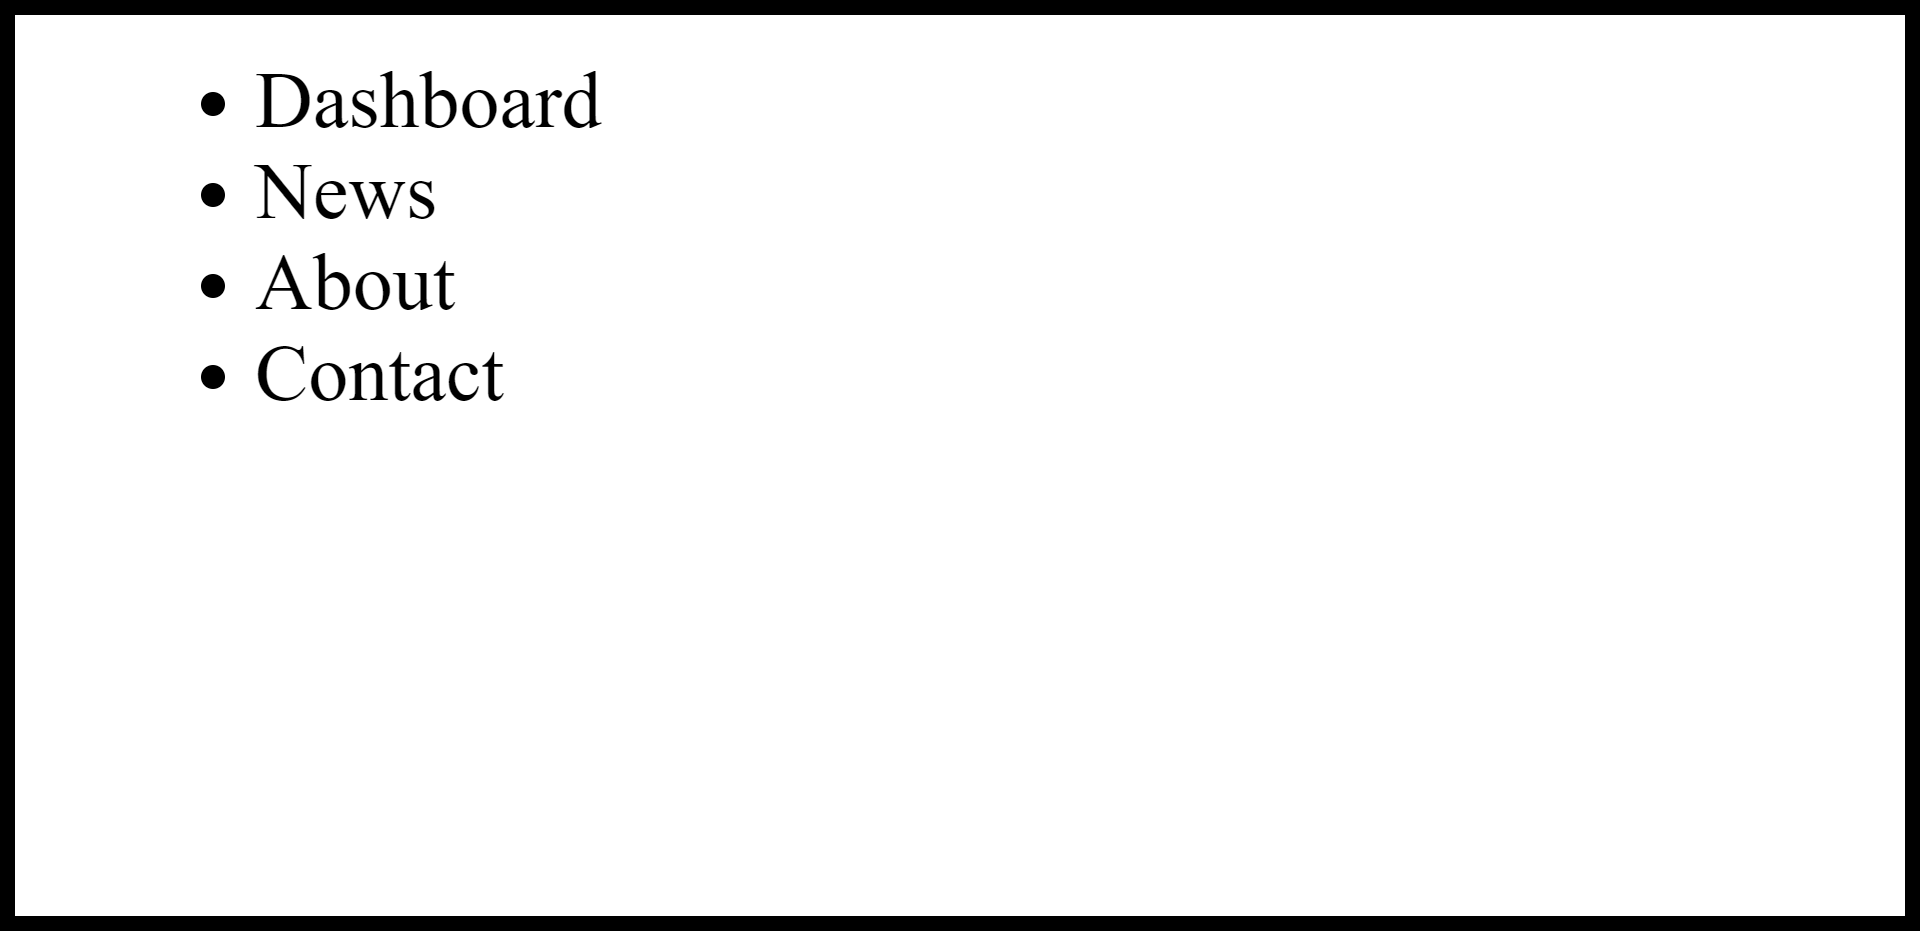
\includegraphics[width=.9\textwidth]{images/figures/fig11.png}

source: %%\url{https://scholar.google.com/citations?view_op=view_citation&hl=id&user=RWuenBkAAAAJ&cstart=20&pagesize=80&authuser=1&citation_for_view=RWuenBkAAAAJ:UeHWp8X0CEIC}
\href{https://scholar.google.com/citations?view_op=view_citation&hl=id&user=RWuenBkAAAAJ&cstart=20&pagesize=80&authuser=1&citation_for_view=RWuenBkAAAAJ:UeHWp8X0CEIC}{Google Scholar}

\end{document}